\section{Experiments: arithmetic gains and recognition regressions}
\label{sec:experiments}

\subsection{Protocol and comparison targets}

The experiment distinguishes three scopes: repeated observations of one actual
suffix, complete raw shadow scans, and the public recognition pipeline. Mixing
these scopes would obscure both the improvement and its limitations.

For repeated observations, the competitors are the maintained direct integer
\code{ClosureShadow}, the earlier rational
\path{determinant_research/boundary_tait.py} prototype, and the new modular
observer with prime 65521. An identical second integer arm controls for ordering
and timing variation. Every arithmetic call constructs a fresh engine and
includes source geometry, response preparation, query processing, and result
collection. No response is warmed outside the timed region.

Each input has one excluded warm-up followed by five rounds with shuffled arm
order. The data retain every elapsed time, arm order, result, input diagram,
crossing order, actual matching stream, source hash, and censoring flag. Very
short pipeline calls use repeated fresh instances and record the individual
call times before forming the round average. Paired speed ratios are formed
\emph{within each round}, then their median is reported. They are not the ratio
of two separately rounded medians.

Each call has a three-second cooperative allowance and a separate 3.15-second
POSIX signal-based wall-clock cap, implemented with \code{SIGALRM} and
\code{setitimer}. The environment is CPython 3.12.14 on Linux x86\_64; the raw file
records the full platform and interpreter strings. Five repetitions support a
local performance comparison, not a distributional or asymptotic claim.
Intervals in the figure are the observed minima and maxima of the five paired
ratios, not confidence intervals.

\subsection{A controlled family of actual query streams}

The base input is a five-strand braid with signed generator indices
\[
 (-2,3,2,2,4,2,-3,-2,-1,1,-2,-1,-2,-2).
\]
Its base crossing order is
\[
 (5,1,10,2,9,11,13,6,7,0,12,4,8,3).
\]
Append $k$ copies of
\[
                         (1,1,-2,-2,3,3,-4,-4)
\]
and place their crossings after the base order. This appended braid is pure:
each generator occurs in an adjacent square, so its permutation is the identity.
The closure therefore keeps the base knot's one-component permutation. The
actual planar diagram is validated as usual.

After the first nine crossings, collect the 200 distinct matchings present in
the real prefix scan. No arbitrary set partitions or invented morphism graph
is substituted for them. This keeps the observation stream tied to the actual
algorithm while increasing the size of the unprocessed interior. The sequence
has $n=5+8k$ suffix crossings and the dimensions in \cref{tab:dimensions}.

\begin{table}[htbp]
\centering\small
\caption{Actual repeated-query suffix dimensions.}
\label{tab:dimensions}
\begin{tabular}{@{}rrrrrrrr@{}}
\toprule
$k$ & $n$ & Queries & $b$ & $v$ & $t$ & $v-t$ & Cofactors\\
\midrule
0 & 5 & 200 & 18 & 9 & 9 & 0 & 61\\
1 & 13 & 200 & 20 & 13 & 10 & 3 & 50\\
4 & 37 & 200 & 20 & 25 & 10 & 15 & 50\\
12 & 101 & 200 & 20 & 57 & 10 & 47 & 50\\
32 & 261 & 50 & 20 & 137 & 10 & 127 & 12\\
\bottomrule
\end{tabular}
\par\smallskip\begin{minipage}{0.97\textwidth}\footnotesize
Here $k$ is the pure-tail repetition count, $n$ the suffix crossings, $b$ the frontier darts, $v$ the common black-fragment vertices, and $t=b/2$ the terminals. Cofactors counts distinct terminal partitions actually evaluated. The last row intentionally uses only the first 50 of 200 available matchings.
\end{minipage}
\end{table}


This family is a controlled arithmetic workload. It is not claimed to be a
hard family for complete unknot recognition, and the fact that its appended
braid is pure does not say that its knot type is unchanged. The fixed source,
not a knot-equivalence claim between rows, defines the experiment.

\subsection{The repeated-query improvement}

\begin{table}[htbp]
\centering\small
\caption{Fresh-setup repeated-query times and paired speed ratios.}
\label{tab:arithmetic}
\begin{tabular}{@{}rrrrrr@{}}
\toprule
$k$ & Integer (s) & Rational (s) & Modular (s) & Int./mod. & Rat./mod.\\
\midrule
0 & 0.008971 & 0.007237 & 0.011583 & 0.670 & 0.608\\
1 & 0.022148 & 0.006680 & 0.011787 & 1.878 & 0.573\\
4 & 0.088640 & 0.014030 & 0.013336 & 6.499 & 1.016\\
12 & 0.734303 & 0.100374 & 0.027537 & 26.666 & 3.968\\
32 & 1.488842 & 1.428603 & 0.138268 & 10.743 & 10.218\\
\bottomrule
\end{tabular}
\par\smallskip\begin{minipage}{0.97\textwidth}\footnotesize
Times are medians of five complete rounds. Ratios are medians of within-round ratios, so they need not equal ratios of the displayed medians. A ratio above one favors the modular evaluator. Prime $65521$ is used throughout.
\end{minipage}
\end{table}


The all-terminal row has no interior work to amortize, and the modular observer
is slower than both predecessors. At three interior vertices it beats the
maintained direct observer but is still slower than the rational prototype.
At 15 interior vertices the rational and modular medians are close. At 47
interior vertices, the modular path gains a median factor of 26.666 over the
direct integer path and 3.968 over the rational prototype. At 127 interior
vertices, the 50-query workload gives factors 10.743 and 10.218 respectively.

The identical-control median ratios in this arithmetic experiment range from
0.953 to 1.036. This supports attributing the larger favorable ratios to a real
change in arithmetic work rather than simply to the order in which the arms
were timed. It does not turn the small-instance ratios into precise universal
constants.

The final row requires a censoring explanation. An initial 200-query pilot at
$k=32$ exhausted the three-second allowance for both direct-integer arms, while
the rational and modular arms completed. That pilot is retained in the raw
record, but no ratio is inferred from its censored times. A separate explicitly
shortened first-50-query workload then completed in all arms and supplies the
reported five-round row. Comparisons within that row are valid; its setup is
amortized over fewer queries than in the preceding rows.

All timed modular interiors have nullity zero. These measurements therefore
support amortization and modular-arithmetic performance, not singular-case
performance. Singular correctness is established by the algebraic and actual-
diagram audits in \cref{sec:implementation}.

\begin{figure}[htbp]
\centering
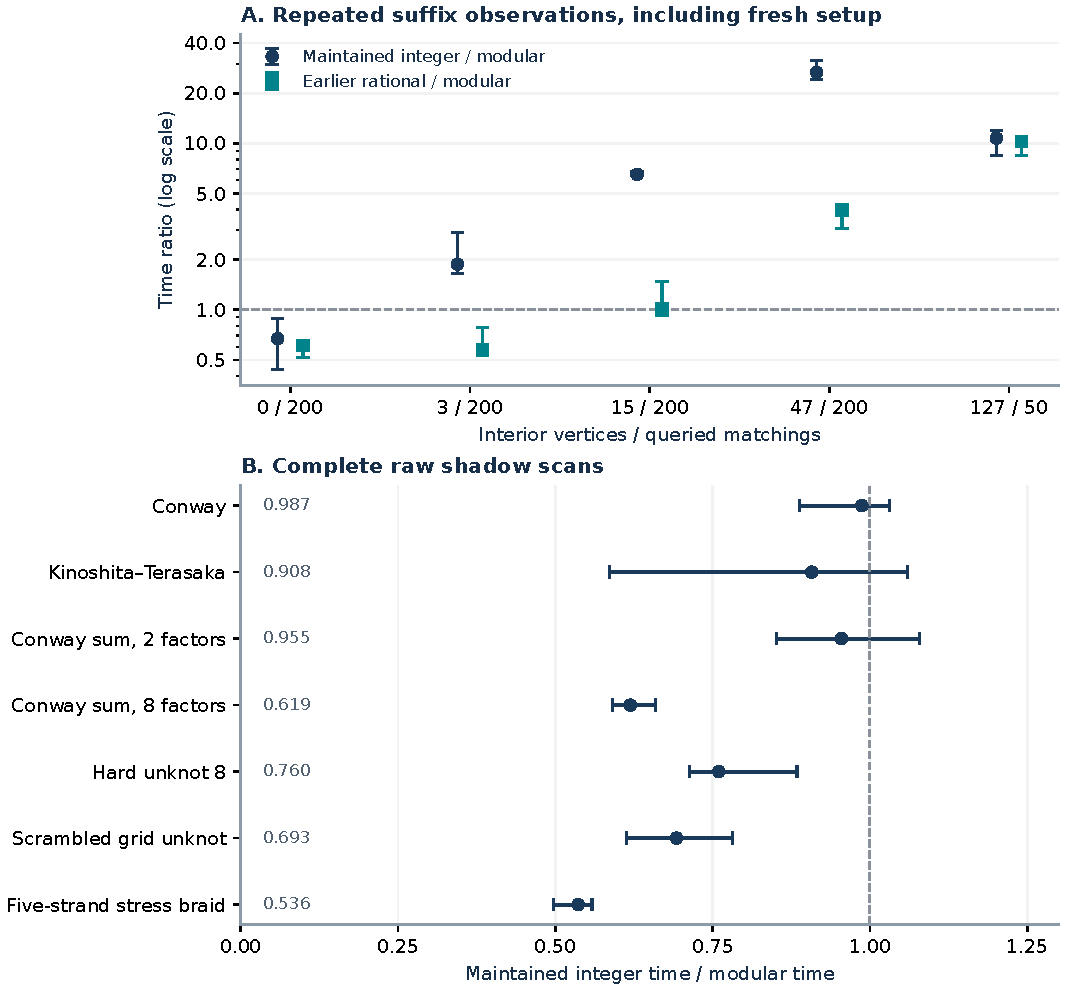
\includegraphics[width=0.99\textwidth]{figures/performance.pdf}
\caption{Measured gains depend strongly on scope. A ratio above one favors the
modular implementation. Points show medians of five paired ratios; whiskers
show the observed range. Panel A includes fresh geometry and response setup.
Panel B measures complete raw scans, where all seven median ratios are below
one. The two panels use different axis scales.}
\label{fig:performance}
\end{figure}

\subsection{The full scans are slower on this corpus}

\begin{table}[htbp]
\centering\small
\caption{The raw scans do not show an overall recognition gain.}
\label{tab:recognition}
\begin{tabular}{@{}lrrrr@{}}
\toprule
Input & Integer (ms) & Modular (ms) & Raw ratio & Filters off\\
\midrule
Conway & 4.774 & 4.895 & 0.987 & 0.969\\
Kinoshita--Terasaka & 5.396 & 5.737 & 0.908 & 0.873\\
Conway sum, 2 factors & 8.807 & 9.494 & 0.955 & 0.961\\
Conway sum, 8 factors & 10.113 & 16.186 & 0.619 & 0.635\\
Hard unknot 8 & 0.972 & 1.264 & 0.760 & 0.803\\
Scrambled grid unknot & 0.513 & 0.741 & 0.693 & 0.677\\
Five-strand stress braid & 1.186 & 2.158 & 0.536 & 0.515\\
\bottomrule
\end{tabular}
\par\smallskip\begin{minipage}{0.97\textwidth}\footnotesize
The first two columns time raw shadow scans. Raw ratio is the paired integer/modular ratio in that scope. Filters off is the corresponding ratio through the public recognition pipeline with its earlier filters disabled. All seven ordinary default-filter runs stop before either shadow backend.
\end{minipage}
\end{table}


The seven examples cover the Conway knot, the Kinoshita--Terasaka knot, visible
connected sums of the Conway knot, two unknot examples, and a five-strand stress
braid. The example names identify the saved input files or generators in the
package; they are not a random sample of knots at those crossing numbers.

Every raw-scan median ratio is below one. The observed range is 0.536--0.987,
with the largest relative regression on the short stress-braid scan. Calling
through the public recognition pipeline with its preceding filters disabled
gives the same qualitative result, with median ratios 0.515--0.969. These
absolute runtimes are short, but the experiment provides no evidence that the
modular backend improves complete scans on this corpus.

The normal pipeline is a separate and especially important control. All seven
examples are decided before either shadow observer is invoked: Conway and
Kinoshita--Terasaka by the modular Jones filter; their visible sums by
factorization followed by that filter; the hard-unknot example by the
three-braid free-product route; the scrambled grid unknot by Reidemeister
reduction; and the stress braid by the modular Alexander filter. Near-one
ratios in those runs measure front-end timing variation. They must not be
reported as evidence for the new continuation.

Across all warm-ups and samples, 24,200 repeated vector comparisons and 2,013
repeated status comparisons agree. These are validation-event counts,
\emph{not} counts of distinct diagrams or completions. Completed integer and
rational vectors agree with the new vectors modulo 65521. Status equality is
required; equality of every stopping stage or intermediate method is not.
The hashed observer sources did not change during the benchmark.

\subsection{The supported performance conclusion}

Boundary reuse removes repeated dependence on a large suffix interior, and
finite-field arithmetic can improve substantially on the rational response
when that interior is large. The production measurements justify keeping this
capability available. The complete-scan results simultaneously show that eager
preparation is not a successful universal policy. A scheduler must estimate
whether a suffix will receive enough distinct useful queries before the scan
moves on or another obstruction succeeds.

The next benchmark should hold out a corpus where the earlier structural,
Alexander, and Jones filters genuinely remain inconclusive, include large
interior graphs with few queries, and measure successful early stops and total
scan work. A claimed default-policy improvement should survive that test with
setup, failed probes, prime refinement, cache memory, and timeouts all charged.
